\documentclass[a4paper,10pt]{article}
\usepackage[utf8x]{inputenc}

\usepackage{amsthm}
\usepackage{amsmath}
\usepackage{amssymb}
\usepackage{geometry}
\usepackage{stmaryrd}

\usepackage[all,cmtip]{xy}
\usepackage{diagxy}
\usepackage{graphicx}

%Set up environments
\theoremstyle{plain}% default
\newtheorem{thm}{Theorem}
\newtheorem{lem}[thm]{Lemma}
\newtheorem{prop}[thm]{Proposition}
\newtheorem{cor}{Corollary}
\theoremstyle{definition}
\newtheorem{defn}{Definition}
\newtheorem{conj}{Conjecture}
\newtheorem{exmp}{Example}
\newtheorem{exer}{Exercise}
\theoremstyle{remark}
\newtheorem{rem}{Remark}

%Useful macros
%Blackboard bold
\newcommand{\NN}{\mathbb{N}}
\newcommand{\ZZ}{\mathbb{Z}}
\newcommand{\RR}{\mathbb{R}}
\newcommand{\CC}{\mathbb{C}}
\newcommand{\HH}{\mathbb{H}}
\newcommand{\QQ}{\mathbb{Q}}

%Specific K-Theory macros (Michal)
\newcommand{\KR}{\widetilde{K}}   % reduced K-theory
\newcommand{\cp}{\CC P}   % complex projective space
\newcommand{\CP}{\cp}     % Rupert prefers capitals...
\newcommand{\CPi}{\cp^\infty}
\newcommand{\smsh}{\wedge}  % shash product of spaces; "wedge" is so confusing and "smash" already exists
\newcommand{\susp}{\Sigma}  % suspension
\newcommand{\htpyequiv}{\simeq}  % homotopy equivalence
\newcommand{\htpic}{\sim}  % homotopic maps
\DeclareMathOperator{\Vect}{Vect}
\renewcommand{\epsilon}{\varepsilon}
\newcommand{\eps}{\epsilon}
\newcommand{\proj}{\mathrm{Proj}}

% Operators
\DeclareMathOperator{\Ker}{Ker}
\DeclareMathOperator{\ch}{ch}

%Arrows
\newcommand{\into}{\hookrightarrow}
\newcommand{\xto}[1]{\xrightarrow{#1}}
\newcommand{\xot}[1]{\xleftarrow{#1}}
\newcommand{\ot}{\leftarrow}



%opening
\title{K - Theory}
\author{Based on lectures by Professor John Jones}

\begin{document}

\maketitle

\tableofcontents

\section{Vector Bundles}

\subsection{Basic Definitions}

K-Theory is principally concerned with the study of vector bundles over topological spaces. So first we cover the basics of vector bundles. 

\begin{defn}
 A real vector bundle over a topological space $B$ is a topological space $E$ and a map $\pi:E\mapsto B$ such that:
 \begin{itemize}
  \item We have the structure of a real vector space on the fibre $E_b:=\pi^{-1}(b)$
  \item The vector bundle locally trivial thus for each $b\in B$ we have a neighbourhood $U\subset B$ 
with $b\in U$ and a homeomorphism $h:U\times \mathbb{R}^n\mapsto E_U := \pi^{-1}(U)$ such that:
  \begin{itemize}
   \item The following diagram commutes:
$$\bfig
\Vtriangle[E`U\times \RR^n`B;h`\pi`\pi_U]
 \efig$$
   \item For all $x\in U$ the natural map $v\mapsto h(x,v)$ is a linear isomorphism.
  \end{itemize}
 \end{itemize}
\end{defn}


The space $E$ is traditionally referred to as the total space, $B$ is referred to as the base space and $\pi$ the projection.

\begin{rem}
 From the local triviality condition we see that the dimension of a fibre is constant on connected components.
In particular if $B$ is connected a vector bundle over $B$ has a well defined dimension. If this dimension is 1
we sometimes refer to the vector bundle as a line bundle.
\end{rem}


\begin{defn}
 A map $\phi:E\mapsto E'$ is a bundle morphism if it takes fibres linearly to fibres thus if:
  \begin{itemize}
   \item The following diagram commutes
$$\bfig
\Vtriangle[E`E'`B;\phi`\pi`\pi'_U]
 \efig$$
   \item For each $b \in B$, $\phi_b:=\phi|_b :E_b \mapsto E'_b$ is a linear map
  \end{itemize}
\end{defn}

As one would expect a sub-bundle of a vector bundle $\pi:E\mapsto B$ is a subspace $E'\subset E$
such that the map induced by the inclusion $i:E'\mapsto E$ is a bundle morphism. Two 
vector bundles $E$ and $E'$ are isomorphic if there is a homeomorphism between them which is a bundle map.
In particular the linear map $\phi_b:=\phi|_b :E_b \mapsto E'_b$ is an isomorphism of vector spaces.

\begin{defn}
  $\Vect(B)$ is the set of isomorphism classes of vector bundles over $B$
\end{defn}

Later we will show that $\Vect(B)$ has some algebraic structure, it is a semi-ring.

\subsection{Examples}

\subsubsection{Product bundles}

Given a topological space $B$ we can see that $B\times \RR^n$ is a vector bundle with projection to
the first coordinate. $B \times\RR^n$ is also known as the trivial bundle and if $E\cong B\times \RR^n$ 
we say that $E$ is trivial.

\subsubsection{Tangent bundle of a sphere}

Take the sphere $S^n$ in $\RR^{n+1}$ then we define:
$$TS^n:=\{(x,v) \in S^n\times \RR^{n+1} | \langle x,v \rangle =0\} $$
Where $TS^n$ is topologised with the subspace topology.
We can see that this is the tangent bundle of $S^n$ and that it is a sub-bundle of $S^n\times \RR^{n+1}$.

\begin{rem}
 This bundle is non-trivial if $n\neq 1,3,7$ this is a deep theorem which while not proved first within 
K-Theory, has it's most elegant proof in this subject.
\end{rem}


\subsubsection{Counterexample}

Consider the following space:
$$W:=\{ (v,w) \in \RR^{n+1}\times \RR^{n+1} | \langle v,w \rangle \}$$
This is not a vector bundle as the preimage of $0$ is the zero vector space but any neighbourhood of $0$ 
contains points with non zero preimage contradicting local triviality.

\subsubsection{Tangent bundle}

We seek to generalise the tangent bundle of a sphere to more general manifolds $M$ embedded in $\RR^N$.
We define the tangent bundle of a manifold by:
$$TM:=\{ (x,v)\in \RR^N\times\RR^N | v\in T_xM \}$$

\begin{rem}
 This definition requires a particular embedding of our manifold in $\RR^N$. There is a more general definition
defined using coordinate charts but it can readily be seen that these definitions give isomorphic bundles. Further 
every manifold of dimension $N$ may be embedded in $\RR^{2N}$ by the Whitney embedding theorem. 
\end{rem}


\subsubsection{Real projective space}

There is an action of $\RR^\ast$ on $\RR^{n+1}$ coming from multiplication. This action restricts to $\pm 1$ on 
the sphere $S^n$ in $\RR^{n+1}$ we define the real projective space as:
$$\RR P^n = \frac{S^n}{\{\pm 1\}} = \frac{\RR^{n+1}\setminus\{0\}}{\RR^\ast}$$
$\RR P^n$ can then be thought of as the set of lines through the origin given a natural topology. This means 
that there is a canonical line bundle where the fibre of a point in $\RR P^n$ is the line in $\RR^{n+1}$ that this 
point represents.
$$K_\RR := \{ ([x],v\in \RR P^n\times \RR^{n+1} | v=tx t\in \RR\}$$

We note that this is non-trivial although we do not have the required machinery to show this yet.

\begin{exer}
 Show that $K_\RR$ is a real 1 dimensional vector space over $\RR P^n$.
\end{exer}


\subsubsection{Other projective spaces}

The entire theory of real vector bundles may be developed over $\CC$ or $\HH$ in exactly the same fashion. This can
be used to define $\CC P^n$ and $\HH P^n$ and canonical complex and quaternionic line bundles over them.

\subsubsection{Grassmannians}

We now want to define the Grassmannian $G_k(\RR^n)$ which will be the set of $k$-dimensional subspaces of $\RR^n$.
This has a canonical $k$-dimensional vector bundle in which the fibre of a point in $G_k(\RR^n)$ is the subspace 
in $\RR^n$ that the point represents. 
To show these actually exist we need to topologise both $G_k(\RR^n)$ and total space of the canonical bundle.
Let $V_k(\RR^n)$ be the space of linear embeddings $\RR^k\mapsto \RR^n$ this has a natural topology as a subspace of
$\RR^{n m}$. Two embeddings $a,b$ in $V_k(\RR^n)$ define the same subspace of $\RR^n$ if there is a $g\in GL_k(\RR)$
with $a=g\cdot b$ thus we define:
$$G_k(\RR^n):=\frac{V_k(\RR^n)}{GL_k(\RR)}$$
And we define the canonical bundle as:
$$U_k(\RR^n):=\{(p,v)\in G_k(\RR^n)\times \RR^n | v\in P\}$$
Then $U_k(\RR^n)$ is a $k$-dimensional vector bundle over $G_k(\RR^n)$ and is non-trivial.

\begin{exer}
Show the following:
 \begin{enumerate}
  \item $G_1(\RR^n)=\RR P^n-1$.
  \item $G_k(\RR^n) = G_{n-k}(\RR^n)$.
  \item $G_k(\RR^n)$ is compact.
  \item Both $V_k(\RR^n)$ and $G_k(\RR^n)$ are smooth.
 \end{enumerate}
What are the dimensions of $G_k(\RR^n)$ and $G_k(\RR^n)$?
\end{exer}

\subsection{Constructions}

\subsubsection{Pullbacks}

Given a vector bundle $\pi:E\mapsto B$ and a map $f:X\mapsto B$ we can form the pullback bundle
$f^\ast E$ over $X$ as follows:
$$f^\ast E := \{ (x,v) \in X\times E | f(x)=\pi(v)\}$$
Then we have that $(f^\ast E)_x=x\times E_f(x)$ and the dimension of $f^\ast E$ is the same as
the dimension of $E$. Further $f^\ast E$ is a vector bundle and $f:X\mapsto Y$ induces a map
$f^\ast \Vect(Y)\mapsto \Vect(X)$ which is functorial thus giving:
\begin{itemize}
 \item $1^\ast = 1$
 \item $(g\circ f)^\ast = f^\ast \circ g^\ast$
\end{itemize}


\subsubsection{Direct Sums}

Given two vector bundles $\pi,\pi':E,E'\mapsto B$ we want to form the direct sum. By which we mean a bundle 
$E\oplus E':\mapsto B$ such that the fibre at a point is the direct sum of the fibres in $E$
and $E'$ respectively thus $(E\oplus E')_x=E_x\oplus E'_x$. We have the following definition:
$$E\oplus E' = \{(v,w)\in E\times E' | \pi(v)=\pi(w) \}$$
If $E\cong F$ and $E'\cong F'$ and $0$ is the product bundle $B\times \RR^0$ then we have the following:
$$ E\oplus E'\cong F\oplus F'$$
$$ E\oplus E'\cong E'\oplus E$$
$$ E\oplus 0\cong E \cong 0\oplus E$$
Thus $\oplus$ extends to give a commutative, associative map with zero on $\Vect(B)$
$$\oplus :\Vect(B)\times \Vect(B)\mapsto \Vect(B)$$
This gives $\Vect(B)$ the structure of an abelian monoid. For example all vector spaces over a point
are product bundles thus we have:
$$\Vect(point)=({\RR^n|n\in\NN},\oplus)\cong (\NN,+)$$

\subsubsection{Tensor Products}

Likewise we would like to define a bundle $E\otimes E'$ such that $(E\otimes E')_x=E_x\otimes E'_x$
We can see that as sets $E\otimes E'=\bigcup_{x\in X}E_x\otimes E'_x$ we wish to define a topology on this.
\begin{enumerate}
 \item We begin with the simplest case that of product bundles. If $E=X\times \RR^n$ and $E'=X\times \RR^m$ 
then we define $E\otimes E = X\times \RR^{n m}$ with the product topology.
 \item Suppose we have isomorphisms $\alpha:X\times\RR^n\mapsto X\times\RR^n$ and 
$\beta:X\times\RR^m\mapsto X\times\RR^m$ we want to check that $\alpha\otimes\beta$ gives an
isomorphism on $X\times(\RR^n\otimes\RR^m)$. This follows as $\alpha(x,v)\mapsto(x,\alpha_x(v))$ where 
$x\mapsto\alpha_x$ is a map from $X$ to $GL_n(\RR)$ and the same for $\beta$. By composition we that that
$$\alpha\otimes\beta(x,v\otimes w)=(x,\alpha_x(v)\otimes\beta_x(w))$$
since the map
$$\otimes:GL_n(\RR)\times GL_m(\RR)\mapsto GL_{n m}(\RR)$$
is continuous. So $\alpha\otimes\beta$ is a bundle morphism and is readily seen to be an isomorphism. 
 \item If $E, E'$ are trivial bundles choice isomorphisms $E\mapsto X\times\RR^n$, $E'\mapsto X\times\RR^m$
then we have a bijection between $E\otimes E'\mapsto X\times\RR^{n m}$ we pullback to get a topology 
on $E\otimes E'$ the previous step sows that this is independent of choices.
 \item To Let $U$ be a set such that $E_U$ and $E'_U$ are trivial and endow $(E\otimes E')_U$ with a topology via the previous
step. To define a topology we say $V\subset E\otimes E'$ is open if and only if $V\cap (E\otimes E')_U$ is open in $(E\otimes E')_U$
for all suitable $U$.
\end{enumerate}


\subsubsection{Other constructions}

We remark that the above construction for tensor products may be carried over for any map $\mathcal{F}:\RR^{n_1}\times\ldots\times\RR^{n_k}\mapsto\RR^m$
for which we have the same continuity condition we used in the proof of the tensor product case.
That the induced map $\mathcal{F}(GL_{n_1}(\RR)\times\ldots\times GL_{n_k}(\RR)\mapsto GL_m(\RR)$ is continuous.


We can then define a bundle $\mathcal{F}(E_1,E_2,\ldots,E_k)$ such that:
$$\mathcal{F}(E_1,\ldots,E_k)_x = \mathcal{F}((E_1)_x,\ldots,(E_k)_x)$$

Some notable examples include
\begin{itemize}
 \item The hom bundle $Hom(E,E')$.
 \item The dual bundle $E^\ast = Hom(E,X\times\RR)$.
 \item Symmetric powers $S^\ast(E)$
 \item Exterior powers $\bigwedge^\ast(E)$
\end{itemize}

\subsection{Algebraic Structure}

Like the direct sum it can be shown that the tensor product operation descends to a map 
$\otimes:\Vect(X)\times \Vect(X)\mapsto \Vect(X)$. This operation is commutative, associative, has a unit element
($\mathbb{1}:=X\times\RR$) and is distributive over $\oplus$. Thus $\Vect(X)$ defines a semi ring. It may also be shown that
pullbacks give semi-ring homeomorphisms thus $\Vect$ gives a functor from topological spaces to semi rings. As an example $\Vect(point)\cong\NN$ the free semi-ring generated by 1 element.


\section{K-Theory}

\subsection{K-Groups}

We would like to extend $\Vect(X)$ so that it has the structure of an ring. We will first extend $\Vect(X)$ to being a
group by adding formal inverses. These new bundles that we add are known as virtual bundles. We will then extend our multiplicative operation $\otimes$ over these virtual bundles to define a ring. In particular after extension $\Vect(point)$ will be 
isomorphic to $\ZZ$.

\begin{defn}
 Given an abelian monoid $A$ then $K(A)$ is the universal abelian group of $A$ if:
 \begin{enumerate}
  \item $K(A)$ is an abelian group.
  \item There exists a morphism of monoids $A\mapsto K(A)$
  \item Given any abelian group $C$ and homomorphism of monoids $\phi:A\mapsto C$ then there exists a unique
group homomorphism $\psi:K(A)\mapsto C$ such that the following diagram commutes:
$$\bfig
\qtriangle[A`K(A)`C;`\phi`\psi]
 \efig$$
 \end{enumerate}
\end{defn}

\begin{rem}
 $K(A)$ is referred to as the $K-group$ or Grothendieck group of $A$.
\end{rem}


We prove existence by giving two constructions of $K(A)$ the first being of more theoretical use, while the second 
is of more practical computational use. Throughout this section we will let $(A,\oplus,\otimes)$ be a semi ring with abelian monoid $(A,\oplus)$ and $K$-group $(K(A),+)$

\subsubsection{Existence}

\begin{enumerate}
 \item Let $(F(A),+)$ be the free abelian group generated by $A$ and define $E(A)$ to be the subgroup of $F(A)$
generated be elements of the form:
$$a+b-(a\oplus b)$$
We then set $K(A):=F(a)/E(A)$.
 \item We define the following relation $\sim$ on $A\times A$
$$(a,b)\sim (c,d) \iff \exists e\in A \mathtt{ with } a\oplus b\oplus e =c\oplus d\oplus e$$
we then set $K(A)=A\times A/\sim$. We denote the equivalence class
\footnote{The notation $K$ derives from the German for class which begins with a K.}
 of $(a,b)\in K(A)$  by $[a,b]$.
Then we define addition in $K(A)$ by:
$$[a,b]+[c,d]=[a\oplus c,b\oplus d]$$
We note that this addition has a zero element $0=[0,0]$ as well as inverses as $[a,b]+[b,a]=0$ and so $[b,a]=-[a,b]$.
We can think of elements in $K(A)$  as formal differences of elements of $A$ in the following way,
the map $[ ]:A\mapsto K(A)$ with $[a]=[a,0]$ gives a homomorphism of monoids such that
$$[a,b]=[a,0]+[0,b]=[a,0]-[b,0]=[a]-[b]$$
\end{enumerate}

\subsubsection{Multiplicative Structure}

We now want to define a multiplicative structure $\times$ on $K(A)$ compatible with $\otimes$ which makes $K(A)$
a ring. As we wish to have $[x]\times[y]=[x\otimes y]$ and a ring structure on $K(A)$ we must have:
\begin{align*}
 [a,b]\times[c,d] &= ([a]-[b])\times([c]-[d])\\
		  &= ([a]\times[c]+[b]\times[d])-([a]\times[d]+[b]\times[c])\\
		  &= ([a\otimes c]+[b\otimes d])-([a\otimes d]+[b\otimes c])\\
		  &= [(a\otimes c)\oplus(b\otimes d)]-[(a\otimes d)\oplus(b\otimes c)]\\
		  &= [(a\otimes c)\oplus(b\otimes d),(a\otimes d)\oplus(b\otimes c)]
\end{align*}

We leave it to reader to show that this structure does give us a ring structure.

\begin{defn}
 Suppose that $X$ is a topological space then we define $K(X)$ to be $K(\Vect(X))$ and we have that the map $X\mapsto K(X)$
is a functor from the category of topological spaces to the category of rings with $K(point)=\ZZ$. We refer to this at the $K$-Theory of a space $X$.
\end{defn}

The object of this course is the study of $K(X)$.

\section{Some Calculations}

Let $X$ be a compact, Hausdorff topological space. We will make use of the following well known results.

\begin{lem}\label{htpyiso}
Suppose $f,g:X\to Y$ are homotopic maps and $E$ is a vector bundle over $Y$. Then $f^*(E)\cong g^* (E).$
\end{lem}

\begin{lem}
For any vector bundle $E$ over $X$ there exists a vector bundle $F$ over $X$ such that $E\oplus F\cong X \times \RR^n.$ 
\end{lem}

\begin{cor}
If $X$ is contractible, then $K(X)\cong \ZZ.$
\end{cor}

Making use of these lemmas we will calculate $K(S^1).$ Note that any vector bundle over $S^1$ can be written as
\[
I \times \RR^n\big/ (0,v) \sim (1,Av)
\]
where $A:0\times \RR^n \to 1\times \RR^n$ is a linear isomorphism sometimes called monodromy.

Let $A$ and $B$ be two monodromies belonging to the same path component of $GL_n(\RR)$ and let $E$ and $F$ be the corresponding vector bundles.  It is easy to see that $E\cong F$. Indeed, using a path joining $A$ and $B$ we can construct a vector bundle over $S^1\times I$ whose restriction to $S^1\times 0$ is $E$ and to $S^1\times 1$ is $F$, then by lemma \ref{htpyiso}, $E\cong F$.

Denote by $\epsilon^n\in \Vect_n(S^1)$ the trivial bundle $S^1\times R^n$ and by $\eta^n$ the other vector bundle of $\Vect_n(S^1)$, corresponding to the monodromy with negative determinant. Since the monodromy corresponding to $\epsilon^n\oplus\epsilon^m$ has positive determinant, we can conclude that $\epsilon^n\oplus\epsilon^m\cong \epsilon^{n+m}.$ Similarly, $\eta^n\oplus\epsilon^m\cong \eta^{n+m}$ and $\eta^n\oplus\eta^m\cong \epsilon^{n+m}.$

Therefore, the monoid $\Vect(S^1)$ is $\NN\times\ZZ/2$ and $K(S^1)=\ZZ\oplus \ZZ / 2.$

\begin{exer}
Find the ring structure of $K(S^1).$
\end{exer}

\begin{rem}
Since $GL_n(\CC)$ is connected $\Vect_n^{\CC}(S^1) = {\epsilon^n}$. Then, $K^\CC (S^1) = \ZZ.$
\end{rem}

\subsection{Constructions on Cones, Suspensions and Loops.}

Let $X$ be a topological space. We will briefly review some basic definitions.

\begin{itemize}
\item The cone of $X$ is $CX=\frac{X\times[0,1]}{X\times 1}.$

\item The suspension of $X$ is $SX = \frac{X \times [-1,1]}{X\times -1\cup X\times +1}.$

\item The base loop space of $X$ is $\Omega (X) =  Map(([0,1],\{0,1\}),(X,x_0)).$

\item $[X,Y]$ denotes the homotopy classes of maps $X\to Y.$
\end{itemize}

\begin{rem}We can see that $SX = C_+X\cup C_- X$ and $X = C_+X\cap C_- X$. Further by constructing for each $f: SX\to Y$ a map $\hat{f}:X\to \Omega Y$ defined by $\hat{f}(x)(t)= f(t,x)$ we conclude that $[SX,Y]\cong [X,\Omega Y]$.
\end{rem}

\subsubsection{The Clutching Construction.}

Suppose $X = X_1 \cup X_2$ and $A= X_1 \cap X_2$. Suppose further that we have two vector bundles $E_1\to X_1$ and $E_2\to X_2$ and an isomorphism $\phi: E_1|_A \to E_2|_A.$
Then space 
\[
E_1\cup_\phi E_2 = \frac{E_1\sqcup E_2}{\sim}
\] 
is a vector bundle, where $u\sim v$ iff $\pi_1(u) = \pi_2(v)\in A$ and $\phi(u)=v$.

\begin{thm}
If $X$ is a connected topological space, then: 
$$\Vect_n(SX) = [X, GL_n(\RR)]$$.
\end{thm}

\begin{proof} Apply the clutching construction to $SX = C_+X\cup C_- X$. Note that $C_+ X$, $C_-X$ are contractible. Choose trivialisations of their trivial bundles $E_+ = E |_{C_+X}\cong C_+X\times \RR^n$ and $E_- = E |_{C_-X}\cong C_-X\times \RR^n.$ Comparing these trivialisations over $X = C_+X\cap C_- X$ gives a map $X\to GL_n(\RR).$

Conversely given a map $f:X\to GL_n(\RR)$ use the clutching construction on $C_+X\times \RR^n$, $C_-X\times \RR^n$ and $\phi:X\times \RR^n\to X\times\RR^n$ defined by $f$. These constructions define inverse isomorphisms.\end{proof}

\begin{cor}
$\Vect_n(S^ k) =  \pi_{k-1}(GL_n(\RR))$
\end{cor}

Returning to the example of the Grassmannians, we have an inclusion
\[ 
i_n:G_k(\RR^n)\to G_k(\RR^{n+1})
\]
and $i_n^*(U_k(\RR^{n+1}))= U_k(\RR^n).$ Let $G_k(\RR^\infty) = \cup_{n=1}^\infty G_k(\RR^n)$ with the direct limit topology, i.e. $V$ is open in $G_k(\RR^\infty)$ if it is open in each element of the union. We can also construct a canonical vector bundle $U_k(\RR^\infty)\to G_k(\RR^\infty)$, the universal bundle.

\begin{thm}
The map
\[
[X,G_k(\RR^\infty)]\to \Vect_k(X)
\] defined by $f\mapsto f^*(U_k(\RR^\infty))$ is a bijection.
\end{thm}

\begin{rem}
Using the previous result for suspensions and the last theorem we have
\[
[SX, G_k(\RR^\infty)] = [X, GL_k(\RR)]
\]
and
\[
[X, \Omega G_k(\RR^\infty)] = [X, GL_k(\RR)].
\]
Indeed there is a homotopy equivalence
\[
\Omega G_k(\RR^\infty) \cong GL_k(\RR).
\]
\end{rem}

\begin{proof}
We will construct an inverse. Let $E\to X$ be a $k$-dimensional vector bundle and choose $F \to X$ such that $E\oplus F \cong X\times \RR^n.$
Define $\Phi_E: X\to G_k(\RR^ n)$ by $x\mapsto E_x\subset \RR^n.$

It is left to the reader to check the continuity of $\Phi_E$ and the identity $\Phi_E^*(U_k(\RR^\infty))= E.$ We must prove that the homotopy class of $\Phi_E$ is independent of the choice of $F$ and of the isomorphism $E\oplus F \cong X\times \RR^n.$

Suppose $i:E\to X\times\RR^n$ and $j:E\to X\times\RR^m$ are two embeddings in a trivial bundle of $x$. Construct the map
$H:[0,1]\times E\to X\times(\RR^n\oplus\RR^m)$ which takes $(t,e)\mapsto (\pi(e),((1-t)i(e),tj(e))).$ Notice that $H$ is an injection because $i$ and $j$ are injections in each fibre. Then $H$ is an embedding in a trivial bundle of $X$.

$H$ induces a map $\overline{H}: I\times X \to G_k(\RR^n\oplus\RR^m)$ such that
the restriction map $\overline{H}|_{{0}\times X}$ is the composition $X \to^{\Phi_{E,i}} G_k(\RR^n) \to^{u_n}  G_k(\RR^n\oplus\RR^m)$ and the restriction map $\overline{H}|_{{1}\times X}$ is the composition $X \to^{\Phi_{E,j}} G_k(\RR^n) \to^{v_m}  G_k(\RR^n\oplus\RR^m)$ with $u_n$ and $v_m$ the inclusions to the the first and second factor, respectively. Then, $u_n\circ \Phi_{E,i} \cong \Phi_{E,j} \circ v_m.$ Observe that if $m,n$ are even then the map $G_k(\RR^n\oplus\RR^m) \to G_k(\RR^n\oplus\RR^m)$ given by permuting the factors is homotopic to the identity. Is left to the reader the case when $m,n$ are odd or have different parity.

This gives a homotopy $\Phi_{E,i}$ to $\Phi_{F,j}.$
\end{proof}

\subsubsection{Important spaces}

The orthogonal group $O_k = \{ A\in GL_k(\RR^n) | AA^t = A^tA = I\}$ is homotopy equivalent to $GL_k(\RR^n).$ Therefore $[X,O_k]=[X,GL_k(\RR^n)] = \Vect_k^\RR(SX).$ Similarly, we have the unitary group $U_k = \{ A\in GL_k(\CC^n) | A\overline{A}^t = A^t\overline{A} = I\}$ and $[X,U_k]= \Vect_k^\CC(SX)$

Let $BO_k = G_k(\RR^\infty)$ and $BU_k = G_k(\CC^\infty)$. Then by the previous theorem we have $[X,BO_k]= \Vect_k^\RR(X)$ and $[X,BU_k]= \Vect_k^\CC(X)$.  Also $\Omega BO_k \cong O_k$ and $\Omega BU_k \cong U_k.$  Since there is an embedding $G_k(\RR^\infty)\to G_{k+1}(\RR^\infty)$ defined by identifying $\RR\oplus\RR^\infty\to \RR^\infty.$ Then define $BO = \cup_{k=1}^\infty G_k(\RR^\infty)$ and $BU = \cup_{k=1}^\infty G_k(\CC^\infty)$.

Given $X$ form $\tilde{K}(X) = \Ker\{dim:K(X)\to K(point) = \ZZ\}.$

\begin{thm}
There are isomorphisms
\[
\tilde{K}^\RR(X) = [X, BO]
\]
\[
\tilde{K}^\CC(X) = [X, BU]
\]
\end{thm}

The proof is going to be discussed later.

\subsection{Bott Periodicity Theorem}

There is an inclusion $O_k\to O_{k+1}$ given by the map
\[A\mapsto \left( 
\begin{array}{cc}
A & 0 \\
0 & 1 
\end{array} \right).\] 
Now form $O = \cup_k O_k\subset M_{\infty,\infty}(\RR),$ the infinite matrices. Observe 
\[O=\bigg\{\left( 
\begin{array}{cc}
A & 0 \\
0 & I_\infty 
\end{array} \right) \bigg| A \text{ finite square matrix}, AA^t = A^tA = I\bigg\}.\] 

We will denote by $K$ to the complex $K-$theory, $K^\CC$ and by $KO$ to the real $K-$theory, $K^\RR.$
\begin{rem}
$\tilde{KO}(S^n) = \pi_n (BO)= \pi_{n-1} (O)$ and
$\tilde{K}(S^n) = \pi_n (BU)= \pi_{n-1} (U).$
\end{rem}

\begin{thm}[Bott Periodicity]
\begin{itemize}
\item $\pi_n(U) \cong \pi_{n+2}(U)$
\item $\pi_n(O) \cong \pi_{n+8}(O)$
\item \[ \pi_n(U) = \begin{cases} 0 & n\text{ even}\\
\ZZ & n\text{ odd}
\end{cases}
\]
\item \[ \pi_n(O) = 
\begin{cases} 
\ZZ / 2 & n\equiv 0\text{mod}8\\
\ZZ / 2 & n\equiv 1\text{mod}8\\
0       & n\equiv 2\text{mod}8\\
\ZZ     & n\equiv 3\text{mod}8\\
0       & n\equiv 4\text{mod}8\\
0       & n\equiv 5\text{mod}8\\
0       & n\equiv 6\text{mod}8\\
\ZZ     & n\equiv 7\text{mod}8.
\end{cases}
\]
\end{itemize}
\end{thm}

In consequence,
\[ \tilde{K}(S^n) = \begin{cases} 0 & n\text{ odd}\\
\ZZ & n\text{ even}
\end{cases}
\]
and \[ \tilde{KO}(S^n) = 
\begin{cases} 
\ZZ / 2 & n\equiv 1\text{mod}8\\
\ZZ / 2 & n\equiv 2\text{mod}8\\
0       & n\equiv 3\text{mod}8\\
\ZZ     & n\equiv 4\text{mod}8\\
0       & n\equiv 5\text{mod}8\\
0       & n\equiv 6\text{mod}8\\
0       & n\equiv 7\text{mod}8\\
\ZZ     & n\equiv 8\text{mod}8.
\end{cases}
\]

\begin{rem}
$\pi_k(O) =\lim_n\pi_k(O_n)=\pi_k(O_N)$ provided that $N>>k$ and 
$\pi_k(U) =\lim_n\pi_k(U_n)=\pi_k(U_N)$ provided that $N>>k.$
\end{rem}

%% Begin lecture 3 (31/01/2012)
\section{Complex K-Theory}

Some of lecture 2 fits under this heading.
We have not yet proved the following two identities.
\begin{align}
  \label{xbu-is-kx} [X, BU] &= \tilde{K}(X)\\
  \label{xu-is-ksx}[X, U] &= \tilde{K}(\Sigma X)
\end{align}
To go about this, note that elements of $K(X)$ are formal differences
$[E]-[F]$, where $E$ and $F$ are vector bundles over $X$. Given two
such expressions, $[E]-[F]$ and $[E']-[F']$, they are equal when there
exists a vector $G$ such that
\begin{equation*}
  E\oplus F' \oplus G \cong E' \oplus F \oplus G
\end{equation*}
It is possible to narrow down the representatives that one has to
consider. Indeed, given bundles $E$ and $F$ (and assuming that $X$ is
paracompact), there is an orthogonal bundle $F^\perp$ such that
$F\oplus F^\perp = X \times \CC^n$ for some integer $n$. Rearranging
this gives that
\begin{equation*}
  [E]-[F] = [E\oplus F^\perp] - n
\end{equation*}
and this shows that any element of $K(X)$ can be written as $[W]-n$
for some vector bundle $W$ on $X$. Here $n$ denotes the trivial bundle
$\eps^n = X\times \CC^n$. When are two such expressions equal?

Two elements of $K(X)$, written as $[W]-n$ and $[W']-n'$, are equal if
and only if there exists a vector bundle $G$ over $X$ such that
\begin{equation*}
  W \oplus \eps^{n'} \oplus G \cong W' \oplus \eps^n \oplus G.
\end{equation*}
Of course, $G$ has an orthogonal complement which can be added to both
sides. Thus $[W]-n = [W']-n'$ if and only if there exists some $L\in
\NN$ such that
\begin{equation*}
  W \oplus \epsilon^{L-n} \cong W' \oplus \epsilon^{L-n'}.
\end{equation*}
This is the definition of $W$ and $W'$ being \emph{stably
  isomorphic}. So we have just proved the following:
\begin{lem}\label{kx-stableisos}
  $\tilde{K}(X)$ is in bijection with the set of stable isomorphism
  class of vector bundles over $X$. The correspondence sends a vector
  bundle $E$ to the formal difference $[E]-n$, where $n$ is the
  dimension of $E$.

  Note that subtracting $n$ here ensures that bundles over a point are
  all sent to zero.
\end{lem}

To interpret this homotopically, remember that complex vector bundles
over $X$ are classified by maps into $BU$. As such, if you start with
an element of $\tilde{K}(X)$, you can apply Lemma \ref{kx-stableisos}
to get a stable isomorphism class of vector bundles. Suppose this is
represented by a vector bundle $E$. Then, if $E$ has dimension $n$, it
is classified by a map $f_E: X \to BU_n$. Composing with the inclusion
$BU_n \into BU$ gives an element of $[X, BU]$.

Obviously, to prove that \eqref{xbu-is-kx} holds, one has to check
that this is a bijection. Suppose that $E$ and $F$ are complex vector
bundles over $X$ of dimension $n$ and $m$, respectively. Denote their
classifying maps by $f_E: X \to BU_n$ and $f_F: X \to BU_m$. Composing
these two with the inclusions of $BU_n$ and $BU_m$ into $BU$ gives two
maps $X\to BU$.

Suppose that these two composite maps are homotopic. Then (because
$BU$ is a direct limit of the $BU_k$'s), there exists some $k$ such that
the two composites
\begin{gather*}
  X \xto{f_E} BU_n \into BU_k\\
  X \xto{f_F} BU_m \into BU_k
\end{gather*}
are homotopic. However, consider $i: BU_n \into BU_{n+1}$. If $V_n$
denotes the universal vector bundle over $BU_n$ then
\begin{equation*}
  i^*(V_{n+1}) = V_n \oplus \eps.
\end{equation*}
As such, the statement that there exists $k$ and a homotopy between
the composites above is the same as saying that
\begin{equation*}
  E \oplus \eps^{k-n} \cong F\oplus \eps^{k-m}.
\end{equation*}
But that's the definition of $E$ and $F$ being stably isomorphic, so
we have proved \eqref{xbu-is-kx}. To prove \eqref{xu-is-ksx}, one can
use a very similar argument.

\section{Cohomological Properties of K-Theory}

Assume throughout this section that $X$ is compact Hausdorff and $A
\subset X$ is some subspace. Start by defining
\begin{equation*}
  \tilde{K}^{-n}(X) = \tilde{K}(\Sigma^n X).
\end{equation*}
Think of this as a reduced cohomology group in negative
dimension. Also define an unreduced relative version by
\begin{equation*}
  K^{-n}(X, A) = \tilde{K}^{-n}(X/A) = \tilde{K}(\Sigma^n (X/A)).
\end{equation*}
As you'd expect, you also define
\begin{equation*}
  K^{-n}(X) = K^{-n}(X, \emptyset).
\end{equation*}
\begin{rem}
  There is a convention here that, for any space $X$, the quotient
  $X/\emptyset$ is $X^+$, the based space consisting of $X$ and a
  disjoint basepoint.
\end{rem}

By Bott periodicity, we know that $K^{-n}(X,A) \cong K^{-n-2}(X,A)$
and so we can extend the definition above to define $K^n(X,A)$ for all
$n \in \ZZ$. There are two points of view:
\begin{enumerate}
\item $K^n(X,A)$ is defined for all integers $n$, and there's an
  isomorphism $K^{n}(X,A) \cong K^{n+2}(X,A)$ for each $n$.

\item There are only really two K-groups: $K^0(X,A)$ and $K^1(X,A)$,
  and they repeat every two dimensions. Explicitly,
  \begin{align*}
    K^0(X,A) &= [X/A, \ZZ\times BU]\\
    K^1(X,A) &= [X/A, U]
  \end{align*}
\end{enumerate}

As a sanity check, we can quickly calculate the K-groups of a point,
$P$. In even dimension (which, taking the second viewpoint above, we
may as well assume to be zero),
\begin{align*}
  K^0(P) = K^0(P, \emptyset) = \tilde{K}^0(P^+) = \tilde{K}^0(S^0)
  = [S^0, \ZZ\times BU] = \pi_0(\ZZ \times BU) = \ZZ.
\end{align*}
To explain the chain of equalities slightly further, first note that
$P^+ \cong S^0$, since they are both just spaces with two
points. Also, the homotopy classes $[S^0, \ZZ\times BU]$ denote based
homotopy classes of based maps, so the $\pi_0$ just comes from the
connected component of $\ZZ\times BU$ that the non-basepoint of $S^0$
is sent to. Finally, $BU$ is connected so there is just one connected
component of $\ZZ\times BU$ for each integer. The odd dimensional
calculation is similar so, skipping some of the steps above, we can
just write:
\begin{equation*}
  K^1(P) = [S^0, U] = \pi_0U = 0.
\end{equation*}

\subsection{The six-term exact sequence}

There is a six-term exact sequence in $K$ theory, which is as follows:
\begin{equation}
  \label{stes}
  \xymatrix{
    K^0(X,A) \ar[r]^{j^*} & K^0(X) \ar[r]^{i^*} & K^0(A)\ar[d]^{\delta}\\
    K^1(A)\ar[u]^{\delta} & K^1(X)\ar[l]^{i^*} & K^1(X,A)\ar[l]^{j^*}
  }
\end{equation}
Here, $i^*$ and $j^*$ just come about from applying the functor $K$
(or $K(\Sigma(-))$) to the inclusions $i: A\to X$ and $j: X\to
(X,A)$).

We will describe $\delta$ in two ways: one is a general homotopical
construction and the other is more geometric via clutching
functions. Proving the exactness of the sequence after defining
$\delta$ is not hard but is tedious, so we won't do that.

\begin{figure}
  \centering
  \label{xcupca}
  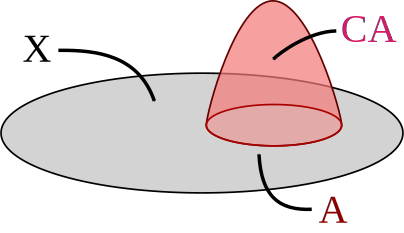
\includegraphics[width=5cm]{img/cone-on-A}
  \caption{$X \cup CA$. Here, $A \cong S^1$ in $X$.}
\end{figure}

Consider the space $X \cup CA$ (depicted in figure
\ref{xcupca}). Collapsing $CA$ to a point gives a map $X\cup CA \to
X/A$ and collapsing $X$ to a point gives a map $X\cup CA \to \Sigma
A$. There is a simple diagram of maps
\begin{equation*}
  \Sigma A \xot{\simeq} (X\cup CA) / X \ot X\cup CA \xto{\simeq} X/A
\end{equation*}
where the two homotopy equivalences shown are indeed homotopy
equivalences as long as $A \into X$ is a cofibration. This is
definitely true if $A$ and $X$ have the homotopy type of
CW-complexes. Inverting the homotopy equivalence on the right and
applying the contravariant functor $\tilde{K}((-)^+)$ gives a map
\begin{equation*}
  K(\Sigma A^+) \to K(X/A^+).
\end{equation*}
This can be used immediately to define a map
\begin{equation*}
  \delta: K^{-1}(A) = \tilde{K}^{-1}(A^+) = \tilde{K}(\Sigma A^+) \to
  \tilde{K}(X/A^+) = \tilde{K}^0(X/A^+) = K^0(X/A)
\end{equation*}
which gives the left hand $\delta$ in \eqref{stes} by Bott
periodicity. To define the $\delta$ on the right (in dimensions of the
other parity), apply the functor $\tilde{K}(\Sigma (-))$ instead and
unpick the relevant definitions. This is quite a general construction:
the connecting homomorphism in the long exact sequence for ordinary
(co)homology can also be defined in terms of this homotopy class of
maps.

Another way to define $\delta$ is via clutching functions. Notice that
an element of $K^0(X,A)$ is a formal difference of bundles over $X/A$
modulo some equivalence relation. Write the set of such classes of
bundles as $\Vect(X,A)$. A class of bundles in $\Vect(X,A)$ can be
represented by a pair consisting of a vector bundle $E$ over $X$ and a
trivialisation of $E$ over $A$. That is, a homeomorphism $\phi:
E|_A\to A\times \CC^n$.

The correct equivalence relation is generated by two types of
equivalence. Firstly, bundles are equivalent if they are stably
isomorphic on $X$. Secondly, they are equivalent if there is a
homotopy between them. That means, for bundles $E_1$ and $E_2$, that
there is a bundle $E$ on $X\times I$ which restricts to $E_1$ at one
end and to $E_2$ at the other such that there is a trivialisation of
the restriction $E|_{A\times I}$.

The direct sum of vector bundles makes the set $\Vect(X,A)$ an abelian
monoid and applying the Grothendieck construction gives
$K^0(X,A)$. Now we want to use a clutching construction...

[Gaargh: I thought I'd finished writing up this lecture but apparently
I haven't. TODO: Beg Robert or others for the end of the notes which I
appear to have lost.]
% End (sort of) lecture 3

\section{Products and operations in $K$-theory}
%% The lecture of 2012.02.07, Scribe: Michal

$K$-theory is equipped with products similar to those in cohomology. The external product of vector bundles composed with diagonal maps $X\to X\times X$ or $X\to X\smsh X$ in the reduced case induces maps
\begin{align*}
K^n(X)\otimes K^m(X)&\to K^{n+m}(X\times X)\to K^{n+m}(X)\\
\KR^n(X)\otimes \KR^m(X)&\to \KR^{n+m}(X\smsh X)\to \KR^{n+m}(X)
\end{align*}
which define the internal product in $K^*(X)$ and $\KR^*(X)$. Note that if $X=\susp Y$ then the product in $\KR(X)$ is trivial, because the diagonal map
$$S^1\smsh Y=\susp Y\to \susp Y\smsh \susp Y=S^1\smsh S^1\smsh Y\smsh Y$$
is the smash of maps $S^1\to S^1\smsh S^1=S^2$ and $Y\to Y\smsh Y$, of which the first one is null-homotopic. In particular, the product in $\KR^*(S^k)$ is always zero.

\subsection{The Kervaire (ups, I meant Hopf) invariant}
Given a map $f:S^{4n-1}\to S^{2n}$ we can form the mapping cone $X=C(f)=S^{2n}\cup_f e^{4n}$. It has one cell in dimensions $0$, $2n$ and $4n$, so by \ref{}  we have $\KR^0(X)=\ZZ\oplus\ZZ$ additively. Let us determine the multiplicative structure.

First, let $i:S^{2n}\hookrightarrow X$ and $q:X\to S^{4n}$ be the canonical maps. For each $k$ choose a generator $\sigma_{2k}\in \KR^0(S^{2k})$. Let $a=q^*(\sigma_{4n})\in\KR^0(X)$ and let $b\in\KR^0(X)$ be any element such that $i^*(b)=\sigma_{2n}$.

We first find
$$a^2=q^*(\sigma_{4n}^2)=0$$
because $\KR(S^{4n})$ has trivial products and $\sigma_{4n}^2\in \KR(S^{4n})$ is zero.

Now note that $ab$ is the image of $b\otimes \sigma_{4n}$ under the map
$$\KR^0(X)\otimes \KR^0(S^{4n})\to \KR^0(X)\otimes \KR^0(X) \to \KR^0(X)$$
which is induced from the map
$$X\to X\smsh X\to X\smsh S^{4n}.$$
But the latter is a map from a space of dimension $4n$ into a space which is $(6n-1)$-connected, so it must be null-homotopic. That means $ab=0$.

It remains to compute $b^2$. Since $a$, $b$ generate $\KR^0(X)$ additively, we have $b^2=\lambda a+\gamma b$, but
$$\gamma=i^*(\lambda a+\gamma b)=i^*(b^2)=\sigma_{2n}^2=0$$
so $b^2=\lambda a$ for some $\lambda\in\ZZ$.

\begin{defn}
The Hopf invariant of a map $f:S^{4n-1}\to S^{2n}$ is the integer $H(f)$ which satisfies $b^2=H(f)a$.
\end{defn}

\begin{exer}
The Hopf invariant has the following properties:
\begin{itemize}
\item[0)] $H(f)$ does not depend on the choice of $b$.
\item[1)] If $f\htpyequiv \susp g$ then $H(f)=0$.
\item[2)] If $f\htpic g$ then $H(f)=H(g)$.
\item[3)] $H:\pi_{4n-1}(S^{2n})\to \ZZ$ is a homomorphism of abelian groups.
\item[4)] There is an element $w_{2n}\in \pi_{4n-1}(S^{2n})$ such that $H(w_{2n})=2$. (Hint: Use $w_{2n}=[\iota_n,\iota_n]$.)
\end{itemize}
\end{exer}


\subsection{Ring structure in $K^*(\cp^n)$}

The purpose of this section is to prove

\begin{thm}
As rings
$$
K^0(\cp^n)=\ZZ[x]/(x-1)^{n+1}
$$
where $x$ is the class of the tautological line bundle over $\cp^n$.
\end{thm}

Of course this result agrees with what the ``even cells'' argument \ref{} tells us about the additive structure. It also follows that $\KR^0(\cp^n)$ is the ideal in $K^0(\cp^n)$ generated by $(x-1)$.

Before the proof let us state a version of the Bott periodicity theorem according to Atiyah. Let $L$ be a complex line bundle over a space $X$. We can form the fibre bundle
$$\pi: P(L\oplus 1)\to X$$
where $P$ denotes the projectivisation. In other words, it is the fibrewise one-point compactification of $L$. This induces a homomorphism
$$\pi^*:K^0(X)\to K^0(P(L\oplus 1))$$
which makes the latter ring into an algebra over $K^0(X)$. Since $P(L\oplus 1)$ it is a projectivisation of a vector bundle, there is a tautological line bundle 
$$H\to P(L\oplus 1).$$

\begin{thm}({\bf Bott periodicity})
There is an isomorphism of rings
$$K^0(P(L\oplus 1))=K^0(X)[h]/(h-1)(lh-1)$$
where $h$ is the class of $H$ in $K^0(P(L\oplus 1))$ and $l$ is the class of $L$ in $K^0(X)$.
\end{thm}

\begin{exmp}
If $L=X\times \CC$ then $P(L\oplus 1)=X\times \cp^1=X\times S^2$ and the theorem takes the familiar form 
$$K^0(X\times S^2)=K^0(X)[h]/(h-1)^2.$$
\end{exmp}

Now we prove, by induction, the ring structure of $K^0(\cp^n)$. Let $K_n\to \cp^n$ denote the tautological line bundle. Then $\cp^n=K_{n-1}^+$ is its one-point compactification. Moreover $P(K_n\oplus 1)$ is the fibrewise one-point compactification of $K_n$ and we have
\begin{equation}\label{eq:pcc}P(K_n\oplus 1)/\cp^{n-1}=\cp^n\end{equation}
define a ring
$$R_n=\ZZ[u,v]/(u-1)^n,(v-1)(u-1).$$
A quick check shows that in $R_n$ we have the identities
$$(v-1)^k=(v-1)(u-1)^{k-1},\quad (v-1)^n\neq 0, \quad (v-1)^{n+1}=0$$
Applying Bott periodicity to the bundle $K_{n-1}\to\cp^{n-1}$ we get
$$K^0(P(K_{n-1}\oplus 1)) = K^0(\cp^{n-1})[v]/(v-1)(lv-1)$$
where $v$ is the class of the tautological bundle over $P(K_{n-1}\oplus 1)$ and $l$ is the class of $K_{n-1}$. But $l$ is invertible in $K^0(\cp^{n-1})$ because $K_{n-1}\otimes K_{n-1}^\ast=\cp^{n-1}\times \CC$ is the trivial bundle. Let $u=l^{-1}$ be the inverse of $l$. Then assuming that we have the result for $K^0(\cp^{n-1})$ we obtain
$$K^0(P(K_{n-1}\oplus 1))=R_n.$$
The inductive step which yields $K^0(\cp^n)$ is now completed using the six-term exact sequence for the pair of \eqref{eq:pcc} and the properties of the ring $R_n$.

\subsection{Natural operations in $K$-theory}

Given an $n$-dimensional complex vector space and an integer $k$ we can form the $k$ exterior and symmetric powers
$$\Lambda^k V=V^{\otimes^k}/(v\otimes w+w\otimes v),\quad S^kV=(V^{\otimes^k})^{\Sigma_n}$$
with $\Lambda^0V=S^0V=\CC$. We can perform the same operations on vector bundles obtaining maps
$$\Lambda^k, S^k:\Vect(X)\to K^0(X).$$
These maps, however, are not additive. For example, the exterior power satisfies
$$\Lambda^k(E\oplus F)=\bigoplus_{i+j=k} \Lambda^i E\otimes \Lambda^j F.$$
Therefore they do not descent to maps $K^0(X)\to K^0(X)$. We are going to use another device to turn them into $K$-theory operations.

Let $t$ be a formal variable and denote
$$\Lambda_t E:=\sum_{i\geq 0} t^i\Lambda^i E\in K^0(X)[[t]].$$
By the previous observations we have $\Lambda_t(E\oplus F)=\Lambda_tE\cdot\Lambda_tF$. As a power series $\Lambda_tE$ starts with $1+\cdots$, so it is invertible. In other words, the image of $\Lambda_t$ lies in the abelian group $G(K^0(X)[[t]])$ of invertible elements, hence the map
$$\Lambda_t:\Vect(X)\to G(K^0(X)[[t]])$$
is a homomorphism of abelian groups (with addition of bundles on the left and multiplication of power series on the right). By the universal property of the Grothendieck construction we obtain a map
$$\Lambda_t:K^0(X)\to G(K^0(X)[[t]])\hookrightarrow K^0(X)[[t]].$$
In a completely analogous way we get maps
$$S_t:K^0(X)\to G(K^0(X)[[t]])\hookrightarrow K^0(X)[[t]].$$
Now we define natural operations $\Lambda^i,S^i:K^0(X)\to K^0(X)$ via
$$\Lambda_t=\sum_{i\geq 0} t^i\Lambda^i,\quad \Lambda_t=\sum_{i\geq 0} t^i\Lambda^i.$$

\begin{exmp}
Let $L$ be a line bundle. Then $\Lambda_tL=1+tL$ and
$$\Lambda_t(-L)=(\Lambda_tL)^{-1}=\frac{1}{1+tL}=\sum_{i\geq 0}(-1)^it^iL^i.$$
From this we read off $\Lambda^i(-L)=(-1)^iL^i$.
\end{exmp}

\begin{exmp}
Let $L$ be a line bundle. Then $S_tL=\sum_{i\geq 0} t^iL^i$ and
$$S_t(-L)=(S_tL)^{-1}=1-tL.$$
From this we read off $S^1(-L)=-L$ and $S^i(-L)=0$ for $i\geq 2$.
\end{exmp}

From the previous examples we see that $\Lambda_{-t}L\cdot S_t L=1$ for a line bundle $L$. This is a general fact.

\begin{prop}
For any vector bundle $E$ we have $\Lambda_{-t}E\cdot S_t E=1$.
\end{prop}
\begin{proof}
By the splitting principle (see below) it is sufficient to check this when $E=L_1\oplus\cdots\oplus L_k$ is a sum of line bundles. But $\Lambda_{-t}$ and $S_t$ are homomorphisms, so
$$\Lambda_{-t}E\cdot S_t E=\prod_{i=1}^k\Lambda_{-t}L_i\cdot S_t L_i=1$$
because we already know the result for a single line bundle $L_i$.
\end{proof}

This was a standard application of the splitting principle, which allows to reduce proofs from arbitrary vector bundles to the case of a sum of line bundles.

\begin{thm}({\bf The splitting principle})
Let $E_1,\ldots,E_m$ be any family of vector bundles over $X$. Then there exists a space $F$ and a map $\pi: F\to X$ such that:
\begin{itemize}
\item $\pi^*: K^0(X)\to K^0(F)$ is an injection
\item for every $i=1,\ldots,m$ the bundle $\pi^*(E_i)$ over $F$ splits into a sum of line bundles.
\end{itemize}
\end{thm}



\subsection{The Adams operations}

We will now define a particularly useful sequence of operations and explain how they are defined in terms of the exterior power operations $\Lambda^i$.

\begin{thm}
There are unique natural operations
$$\psi^k: K^0(X)\to K^0(X), \quad k\geq 0$$
such that
\begin{itemize}
\item $\psi^k(x+y)=\psi^k(x)+\psi^k(y)$,
\item if $L$ is a line bundle then $\psi^k(L)=L^k$,
\item $\psi^k\psi^l(x)=\psi^{kl}(x)$,
\item $\psi^k(xy)=\psi^k(x)\psi^k(y)$.
\end{itemize}
\end{thm}

\begin{rem}
  We note that the final remark makes sense and is true for both the internal
  and external products.
\end{rem}

\begin{proof}(Sketch)
The uniqueness part follows from the first two conditions and the splitting principle. To show existence we first define $\psi_t(x)\in K^0(X)[[t]]$ by the formula
\begin{align*}
\psi_{-t}(x)&= \dim(x)-\frac{t}{\Lambda_t(x)}\frac{d}{dt}\Lambda_{t}(x)\\
&= \dim(x)-t\frac{d}{dt}\log(\Lambda_{t}(x))
\end{align*}
and then set 
$$\psi_t(x)=\sum_{i\geq 0}t^i\psi^i(x).$$
\end{proof}

\begin{exmp}
We can calculate how the Adams operations depend on the $\Lambda^i$:
\begin{itemize}
\item $\psi^1-\Lambda^1=0$
\item $\psi^2-\psi^1\Lambda^1+2\Lambda^2=0$
\item $\cdots$
\item $\psi^k-\psi^{k-1}\Lambda^1+\cdots\pm\psi^1\Lambda^{k-1}+(-1)^kk\Lambda^k=0$

\end{itemize}
\end{exmp}


For $k\geq n$ elementary algebra shows that:

\begin{align*}
  \Phi_1-\sigma_1&=0\\
  \Phi_2-\Phi_1\sigma_1+2\sigma_2&=0\\
  \Phi_3-\Phi_2\sigma_1+\Phi_1\sigma_2-3\sigma_3&=0\\
  \cdots \text{etc}
\end{align*}

Where we define $\Phi_i$ by:

$$\Phi_i(x_1,\cdots ,x_n)=x_1^i+\cdots +x_n^i$$

and $\sigma_i$ are the elementary symmetric functions which are defined by the
power series:

$$(1+t x_1)\cdots (1+t x_n)=\sum t^i\sigma(x_1,\cdots ,x_n)$$

The correspondence between these two is easy to show on sums of line bundles and
follows in general by naturality and the splitting principle.

Given line bundles $x_1,\cdots x_n\in K(X)$ and $x=x_1+,\cdots x_n$ we have

$$\Psi^k(x)=x_1^k+\cdots x_n^k = \Phi(x_1,\cdots ,x_n)$$

by the definition we also have that $\Lambda_t(x)=(1+t x_1)\cdots (1+t x_n)$ and so
$\Lambda^i(x)=\sigma(x_1,\cdots x_n)$.

\begin{defn}
  Given $x,y\in K(X)$ then $x=y \mod p$ for some $p\in \ZZ$ if there exists
  $b\in K(X)$ such that $x=y+p b$.
\end{defn}

\begin{lem}
  Suppose that $p$ is prime then for $x\in K^0(X)$ we have:
$$\Phi^k(x)=x^p \mod p$$
\end{lem}

\begin{proof}
  We argue by power series, first we note that $(x+y)^p=x^p+y^p \mod p$ as the 
  $i^{th}$ coefficient in the expansion of $(x+y)^p$ is $\frac{p!}{(p-1)!i!}$ which is
  divisible by $p$ if $i$ is not 0 or $p$. This give us:
$$x_1^p + \ldots + x_n^p=(x_1+\ldots+x_n)^p + p f(\sigma_1,\ldots \sigma_n)$$
Now suppose $E$ is a sum of line bundles over $X$ then we get:
$$\Psi(E)=E^p+p f(\Lambda^1(E),\ldots,\Lambda^n(E))$$
Which proves the lemma by the splitting principle as $f$ is natural.
\end{proof}

\begin{lem}
Let $\Psi^k$ be the Adam's operation $\Psi^k:\KR^0(S^{2n})->\KR^0(S^{2n})$ then
$\forall u\in \KR^0(S^{2n})$ we have $\Psi^k(u)=k^nu$. 
\end{lem}

\begin{proof}
  We first prove the case where $n=1$. If $k$ is the tautological line
  bundle on $S^2$ and $x=[k]$ then we have $K^0(S^2)=\frac{\ZZ[x]}{(x-1)^2=0}$
  and $\KR^0(S^2)$ is the ideal generated by $x-1$. So we only need to show
  the result for $\alpha=x-1$:
\begin{align*}
  \Psi^k(\alpha)=\Phi^k(x-1)&=x^k-1^k\\
  &= (1+\alpha)^k - 1\\
  &= 1+k\alpha-1 = k\alpha
\end{align*}
Where the transition from the second to third line comes from the fact that
$\alpha^k=0$ for $k\neq 0,1$. In the general case we use the Bott periodicity isomorphism
$\KR^0(S^2)\otimes\KR^0(X)\cong K^0(S^2\smsh X)$. So
$\KR^0(S^{2n})\cong\KR^0(S^{2n-2}\smsh S^2)$ is generated by
$\alpha\ast\beta$ with $\alpha\in\KR^0(S^2)$ and $\beta\in\KR^0(S^{2n-2})$. Assume the result holds for $n-1$ then:
\begin{align*}
  \Psi^k(\alpha\ast\beta)&=\Psi^k(\alpha)\ast\Psi^k(\beta)\\
  &=k\times k^{n-1}(\alpha\ast\beta) = k^n(\alpha\ast\beta)
\end{align*}
\end{proof}

\subsection{Hopf Invariant}

We now use Adam's operations to give a proof of Adam's theorem on odd Hopf
invariants.

\begin{thm}
  If $H(f)$ is odd then $n=1,2,4$.
\end{thm}

\begin{proof}
  We recall our notation from earlier, let $\sigma_{2n}$ be a chosen set of generations for
  $\KR^0(S^{2n})$. Then we define $a=p^*\sigma_{4n}$ and choose $b$ such that
  $i^*b=\sigma_{2n}$. We proved that $a^2=a b=0$ and $b^2=H(f)a$. 
  We now assume  that $H(f)$ is odd and compute the Adam's operations.
  \begin{align*}
    \Psi^k(a)=\Psi^k(p^*\sigma_{4n})&=p^*\Psi^k(\sigma_{4n})\\
    &=p^*(k^{2n}\sigma_{4n})=k^{2n}a
  \end{align*}

$$ i^*\Psi^k(b)=\Psi^k(i^*b)=\Psi^k(\sigma_{2n})=k^n\sigma_{2n}$$
Thus for some $\mu_2,\mu_3\in\ZZ$ we have
\begin{align*}
  \Psi^2(b)&=2^nb+\mu_2a\\
  \Psi^3(b)&=3^nb+\mu_3a
\end{align*}
This gives
\begin{align*}
  \Psi^3\Psi^2(b)&=\Psi^3(2^nb+\mu_3a)\\
  &=2^n(3^nb+\mu_3a)+3^{2n}\mu_2a\\
  &=6^nb+(2^n\mu_3+3^{2n}\mu_2)a\\
  \Psi^2\Psi^3(b)&=\Psi^2(3^nb+\mu_2a)\\
  &=3^n(2^nb+\mu_2a)+2^{2n}\mu_3a
  &=6^nb+(3^n\mu_2+2^{2n}\mu_3)a
\end{align*}
By the commutativity of $\Psi$ we get
$2^n\mu_3+3^{2n}\mu_2=3^n\mu_2+2^{2n}\mu_3$ which implies
$3^n(3^n-1)\mu_2=2^2(2^2-1)\mu_3$. As $\Psi^2(b)=b^2 \mod 2 = H(f)a \mod 2$ we
get that $\mu_2$ and hence $\mu_3$ is odd. This implies that $2^n|(3^n-1)$ and
our prove will be completed with the following number theory lemma and it's corollary.

\begin{lem}
  Define $\nu(k)$ by $k=2^{\nu(k)}l$ for $l$ odd. Then $\nu(3^n-1)$ is given
  by:

  \begin{enumerate}
  \item $\nu(3^n-1)=1$ for $n$ odd.
  \item $\nu(3^n-1)=3$ for $n=2$ mod 4.
  \item $\nu(3^n-1)=1+\nu(3^{n/2}-1)$ if $n=0$ mod 4.
  \end{enumerate}
\end{lem}

\begin{proof}
We prove each case of the result:
  \begin{description}
    \item[$n=2k+1$]
      As $3=-1 \mod 4$ and $n$ is odd $3^n=-1 \mod 4$ thus $3^n-1=2 \mod 4$
      and so $3^{2k}+1-1$ is equal to twice an odd number.
    \item[$n=4k+2$]
      We have $3^n-1 = (3^{2k+1}-1)(3^{2k+1}+1)$ where from the last part we
      know that $(3^{2k+1}-1)$ is twice an odd number. As $(3^{2k+1})+1=4 \mod
      8$ we see that $(3^{2k+1})+1$ is 4 times an odd number and the result
      follows.
    \item[$n=4k$]
      We have that $3^n-1=(3^{2k}-1)(3^{2k}+1)$ and
      $\nu(3^n-1)=\nu(3^{n/2}-1)+\nu(3^{2k}+1)$ so it remains to show that
      $\nu(3^{2k}+1)=1$ which follows as $3^{2k}+1 = 2 \mod 8$.
  \end{description}
  
\end{proof}

\begin{cor}
  If $2^n|(3^n-1)$ then $n=1,2,4$.
\end{cor}

\end{proof}

\subsection{Leray Hirsch Theorem in K - Theory}

Suppose that $f:X\mapsto Y$, $U\subset Y$ and let $X_U=f^{-1}(U)$ Suppose in
addition that we have homogeneous elements $\beta_1,\ldots ,\beta_n\in
K^*(X)$.
Let $B^*$ be the free graded abelian group generated by the $\beta_i$ where
$B^*=B^0\oplus B^1$ is its decomposition into homogeneous components.
Then we get a homeomorphism
\begin{align*}
  K^*(U)\otimes B^* &\mapsto K^*(X_U)\\
  x\otimes \beta_j  &\mapsto f_U^*(x)i_U^*(\beta_j)
\end{align*}
Where $f_U$ is the restriction of $f$ to $U$ and $i_U$ is the inclusion. Given
$V\subset U$ we get the following diagram:

$$\bfig
  \Square[K^*(U)\otimes B^*`K^*(U)`K^*(V)\otimes B^*`K^*(V); ` ` ` `]
  \efig$$


\begin{defn}
  Let $f:X\mapsto Y$ be a map then:
  \begin{itemize}
  \item $f$ is a product in K-Theory over $U$ if for all $V\subset
    U$ we have $K^*(V)\otimes B^*\mapsto K^*(X_V)$.
  \item $f$ is a product in K-Theory if it is a product over $Y$.
  \item $f$ is locally a product is for all $y\in Y$ there is an
    open neighbourhood $U\subset Y$ with $f$ a product over $U$.
  \end{itemize}
\end{defn}

\begin{thm}\label{local-to-global-product}
  Assume $Y$ is compact and $f:X\mapsto Y$ is locally a product in  K-Theory
  then $f$ is globally a product
\end{thm}

The proof will require the following lemma the proof of which follows from the
5-lemma and the 6-term exact sequence and is left as an exercise.

\begin{lem}
  Let $f:X\mapsto Y$ and $V\subset U\subset Y$ then if any 2 of
  $\mu_U,\mu_V,\mu_{U,V}$ are isomorphisms then they all are.

$$\bfig
\vSquares[K^*(V)\otimes B^*`K^*(X_V)`K^*(U)\otimes
B^*`K^*(X_U)`K^*(U,V)\otimes B^*`K^*(X_U,X_V);\mu_V` ` `\mu_U` ` `\mu_{U,V}]
\efig$$
\end{lem}

\begin{proof}[Proof of Theorem]
  By compactness it is enough to show that $f$ if is locally a product over
  $U_1,U_2$ then it is also locally a product over $U_1\cup U_2$. Given
  $V\subset U_1\cup U_2$ choose $V_1\subset U_1, V_2\subset U_2$ with $V_1\cup
  V_2=V$ then we have $\frac{V}{V_2}=\frac{V_1}{V_1\cap V_2}$ and
  $\frac{X_V}{X_{V_2}}=\frac{X_v1}{X_{V_1\cap V_2}}$. Which gives us that

  $$\bfig
    \Square[K^*(V,V_2)\otimes B^*`K^*(V_1,V_1\cup V_2)\otimes
    B^*`K^*(X_V,X_{V_2})`K^**(X_{V_1},X_{V_1\cup V_2});\cong`\mu`\cong \text{By lemma} `\cong]
  \efig$$
  Thus $\mu$ is an isomorphism. We now apply the lemma again to get that
  $K(V)\otimes B^*\mapsto K(X_V)$ is an isomorphism as $K(V_1,V_2)\otimes B^*\mapsto
  K(X_{V_1,V_2})$ and $K(V_2)\otimes B^*\mapsto K(X_{V_2})$ are isomorphisms. This finished
  the proof.
\end{proof}

% Lecture of 28/2/2012: Part 2 of the Leray Hirsch theorem story, I
% think.
\subsection{Generalised Cohomology Theories}

A \emph{generalised cohomology theory} consists of the following data:
\begin{itemize}
\item For each $q \in \ZZ$ and (suitable: see below) pair of spaces
  $(X,A)$, an abelian group $E^q(X,A)$. Write $E^q(X)$ for the group
  $E^q(X, \emptyset)$.

\item For every map of pairs $(X,A) \xto{f} (Y,B)$, and for each $q
  \in \ZZ$, an induced homomorphism of abelian groups $f^*: E^q(Y,B)
  \to E^q(X,A)$.

\item A homomorphism $\Delta: E^q(A) \to E^{q+1}(X,A)$, called the
  connecting homomorphism.
\end{itemize}
These data must satisfy the following axioms (the Eilenberg--Steenrod
axioms, minus the dimension axiom):
\begin{enumerate}
\item If $f: (X,A) \to (X,A)$ is the identity then $f^*$ is the
  identity on $E^q(X,A)$ for each $q$.

\item Given $f: (X,A)\to (Y,B)$ and $g: (Y,B)\to (Z,C)$, the
  composites before and after applying $E^q$ are related by $(gf)^* =
  f^*g^*$.

\item \emph{Naturality of the connecting homomorphism}. If $f:
  (X,A)\to (Y,B)$ is a map of pairs then the following diagram
  commutes.
  \begin{equation*}
    \xymatrix{
      E^q(A) \ar[r]^-\Delta & E^{q+1}(X,A)\\
      E^q(B) \ar[r]_-\Delta \ar[u]^{(f|_A)^*} & E^{q+1}(Y,B) \ar[u]_{f^*}
    }
  \end{equation*}
  where the $\Delta$ on the top line is that for the pair $(X,A)$ and
  the $\Delta$ on the bottom line is for the pair $(Y,B)$.

\item \emph{Homotopy invariance}. Given maps $f$ and $g$ such that $f
  \simeq g$, it follows that $f^* = g^*$.

\item \emph{The exact sequence of a pair}. Given a pair of spaces
  $(X,A)$, let $p: (X,\emptyset) \to (X,A)$ and $i: A \into X$. Then
  the following sequence is exact.
  \begin{equation*}
    \dots \to E^{q-1}(A) \xto{\Delta} E^q(X,A) \xto{p^*}
    E^q(X) \xto{i^*} E^q(A) \xto{\Delta} E^{q+1}(A) \to \dots
  \end{equation*}

\item \emph{Excision}. The natural map $(X,A) \to (X/A, *)$ (where $*$
  denotes the image of $A$ in $X/A$) induces isomorphisms $E^q(X/A,*)
  \to E^q(X,A)$.
\end{enumerate}
The last axiom, explains the data above asked for ``suitable''
spaces. In general, one can only expect this to work when the
inclusion $A \into X$ is a cofibration. This is true for $X$ a CW
complex and $A$ a subcomplex. By Whitehead's theorem (which says that
any map between spaces can be represented up to weak equivalence by a
CW map between CW complexes), it suffices to define $E^*$ on such
spaces and maps.

A \emph{natural transformation} of cohomology theories $\phi^*: E^*
\to F^*$ is defined to be a sequence of homomorphisms
\begin{equation*}
  \phi^q_{(X,A)}: E^q(X,A) \to F^q(X,A)
\end{equation*}
such that naturality diagrams commute for induced homomorphisms and
also for $\Delta$.

\begin{thm}[Eilenberg-Steenrod]
  Suppose that $\phi^*: E^*\to F^*$ is a natural transformation of
  cohomology theories and that $\phi^q_{pt}: E^q(pt)\to F^q(pt)$ is an
  isomorphism for all $q$. Then $\phi^q_{(X,A)}: E^q(X,A)\to F^q(X,A)$
  is an isomorphism for all pairs of spaces $(X,A)$ and integers $q$.
\end{thm}

Note that this only applies if a natural transformation $\phi$ exists
with the given behaviour on points. For example, one can define a
theory
\begin{equation*}
  E^*(X,A) = H^*(X,A)\otimes \ZZ[u,u^{-1}],
\end{equation*}
where $u$ has degree $2$ and $\otimes$ denotes the tensor product of
graded abelian groups. Although $E^*$ has the same groups as $K^*$ on
a point, the theories are not isomorphic.

Here is a sketch proof of the theorem: Firstly, $E^*(S^0)\to F^*(S^0)$
is an isomorphism (use the exact sequence of the obvious pair and the
five lemma). Next, use the exact sequence again to show that
\begin{equation*}
  E^*(D^1,S^0) \to F^*(D^1,S^0)
\end{equation*}
is an isomorphism. By excision, conclude that $E^*(S^1)\to F^*(S^1)$
is an isomorphism. Now do a similar trick to show by induction that
every $E^*(S^n)\to F^*(S^n)$ is an isomorphism. Now suppose that
$E^*(X)\to F^*(X)$ is an isomorphism. If $f: S^{k-1}\to X$ and
$Y=X\cup_f D^k$ then use an exact sequence (the Mayer-Vietoris
sequence, in fact) to show that $\phi*$ is an isomorphism for
$Y$. Finally, every CW complex can be built inductively by attaching
cells to $S^0$ in this fashion.

An application of this theorem is the following lemma
\begin{lem}\label{kxcpn-kunneth}
  The product map $K^*(X)\otimes K^*(\CP^n) \to K^*(X\times \CP^n)$ is
  an isomorphism.
\end{lem}
\begin{proof}
  Firstly, define a cohomology theory by $E_1^*(X,A) = K^*(X,A)\otimes
  K^*(\CP^n)$. When checking the axioms, it's important that
  $K^*(\CP^n)$ is torsion-free, so tensoring with it preserves the
  exact sequence of a pair from $K^*(X,A)$. Note that this also shows
  what the connecting homomorphism must be: $\Delta_K\otimes 1$.

  Next (much easier), $E_2^*(X,A) = K^*(X\times \CP^n, A\times \CP^n)$
  also defines a cohomology theory. The product map is then a natural
  transformation of cohomology theories $E_1^*\to E_2^*$ and is
  clearly an isomorphism when $X$ is a point.
\end{proof}

Now it is possible to prove the Leray-Hirsch theorem in K-theory:
\begin{thm}[Leray-Hirsch]
  \label{leray-hirsch}
  Let $E$ be a (complex) vector bundle over a compact space $X$ and
  $P(E)$ be its projective bundle. Write $K$ for the tautological
  bundle over $P$ and define $x = [K] - 1 \in K^*(P(E))$. Then
  $K^*(P(E))$ is a free module over $K^*(X)$ with basis $1,x,x^2,\dots
  x^{n-1}$ where $n$ is the dimension of $E$.
\end{thm}
\begin{proof}
  Notice that the projection $\pi: P(E)\to X$ induces a ring
  homomorphism
  \begin{equation*}
    \pi^*: K^*(X)\to K^*(P(E)).
  \end{equation*}
  As normal, this gives $K^*(P(E))$ the structure of a $K^*(X)$
  module. The conclusion can be restated as ``$\pi$ is globally a
  product in K-theory'' (and this is the way to prove it). By Theorem
  \ref{local-to-global-product}, it suffices to show that $\pi$ is
  locally a product in K-theory. Now, given $x\in X$, choose a
  neighbourhood $U$ of $x$ such that
  \begin{equation*}
    E|_U \cong U \times \CC^n.
  \end{equation*}
  Then the projective bundle is simply
  \begin{equation*}
    P(E)|_U \cong U \times \CP^{n-1}.
  \end{equation*}
  Now apply the K\"unneth formula from Lemma \ref{kxcpn-kunneth},
  which shows that $\pi$ is a product in K-theory over $U$.
\end{proof}
Note that this argument only really needs the K\"unneth formula to
work. In particular, this theorem is definitely also true for ordinary
cohomology, $H^*$, as well.

\subsection{The Splitting Principle in K-theory}

\begin{thm}[Splitting Principle]
  Let $E$ be a (complex) vector bundle over $X$. Then there exists a
  space $F$ together with a map $f: F\to X$ such that
  \begin{enumerate}
  \item The induced map $f^*: K(X) \to K(F)$ is injective.
  \item The pullback bundle, $f^*(E)$, is isomorphic to a sum of line
    bundles.
  \end{enumerate}
\end{thm}
\begin{proof}
  (A sketch.) Start with $F_1 = P(E)$ and $\pi_1: P(E)\to X$. By the
  Leray-Hirsch theorem, $\pi_1^*$ includes $K^*(X)$ as the
  $K^*(X)\cdot 1$ summand. In particular, it is injective. But the
  tautological bundle $K$ is a sub-bundle of $\pi_1^*(E)$, so
  $\pi_1^*(E) \cong K\oplus E'$ where $E'$ has dimension one less than
  that of $E$. This is the inductive step.
\end{proof}

\section{The Chern Character}

The objective of this section is to construct a natural transformation
of cohomology theories
\begin{equation*}
  \ch: K^*(X)\otimes \QQ \to H^*(X; \QQ)
\end{equation*}
called the \emph{Chern character}. To be precise, collect up even and
odd terms of the rational cohomology ring as
\begin{align*}
  H^{ev}(X; \QQ) &= \prod_n H^{2n}(X; \QQ)\\
  H^{odd}(X; \QQ) &= \prod_n H^{2n}(X; \QQ)
\end{align*}
(This really is a product, rather than a direct sum. If $X$ has the
homotopy type of a finite dimensional CW complex, the product is
finite, so isomorphic to a direct sum, but this is not true for
general spaces). The natural transformation $\ch$ will map
\begin{align*}
  K^0(X)\otimes \QQ &\to H^{ev}(X; \QQ)\\
  K^1(X)\otimes \QQ &\to H^{odd}(X; \QQ)
\end{align*}

First, however, is a quick diversion to the theory of characteristic
classes. Start with the set of line bundles on a space $X$. So far, it
has had several names:
\begin{equation*}
  \mathcal{L}(X) = \Vect_1(X) = [X, G_1(\CC^\infty)] = [X, \CPi]
\end{equation*}
and the last definition is the one that we need for now.

The cohomology of $\CPi$ is given by $H^*(\CPi; \ZZ) = \ZZ[u]$, where
$u\in H^2(\CPi;\ZZ)$. Given a line bundle $L$ over $X$, write $\phi_L:
X\to \CPi$ for its classifying map (defined up to homotopy). The
\emph{first Chern class}, $c_1(L)$ is defined by
\begin{equation}\label{eq:first-chern-class}
  c_1(L) = \phi_L^*(u) \in H^2(X; \ZZ).
\end{equation}
The first Chern class has the following properties:
\begin{enumerate}
\item $c_1(f^*L) = f^*c_1(L)$ (because $\phi_{f^*L} \simeq \phi_L
  \circ f$)

\item If $L \cong L'$ then $c_1L = c_1L'$ (because the classifying
  maps of the line bundles are homotopic, so $H^*$ takes the same
  value on both).
\end{enumerate}
The tensor product of line bundles, $\otimes$, makes the set of line
bundles on $X$ a group. The unit is the trivial line bundle $\epsilon
= X\times \CC$ and the inverse of a bundle $L$ is the dual bundle,
$L^*$.

\begin{thm}
  $c_1: \mathcal{L}(X) \to H^2(X;\ZZ)$ is an isomorphism of groups.
\end{thm}
\begin{proof}
  Here, we shall prove that $c_1$ defines a homomorphism. See previous
  TCC course or a textbook.
  %% TODO:
  %%   Which one? Neither Milnor and Stasheff nor Atiyah
  %%   (K-Theory) seem to prove this(!)
  Starting with $K$ the tautological bundle, consider $K \boxtimes K$,
  the external tensor product of $K$ with itself. The classifying map
  of $K\boxtimes K$ defines a map (up to homotopy)
  \begin{equation*}
    \mu: \CPi\times\CPi \to \CPi.
  \end{equation*}
  By the K\"unneth formula (in ordinary cohomology),
  \begin{equation*}
    H^2(\CPi\times \CPi) = H^2(\CPi)\otimes H^0(\CPi) \oplus
    H^0(\CPi)\otimes H^1(\CPi),
  \end{equation*}
  which has a basis $u\otimes 1$, $1 \otimes u$. It is a fact (which
  we shall not prove) that
  \begin{equation*}
    \mu^*(u) = u\otimes 1 + 1 \otimes u.
  \end{equation*}
  As such, if $L$ and $L'$ are line bundles then the classifying
  map of $L\otimes L'$ is
  \begin{equation*}
    X \xto{\Delta} X\times X \xto{\phi_{L}\times \phi_{L'}}
    \CPi\times \CPi \xto{\mu} \CPi
  \end{equation*}
  and, in cohomology,
  \begin{equation*}
    c_1(L) + c_1(L') \mapsfrom
    c_1(L)\otimes 1 + 1 \otimes c_1(L') \mapsfrom
    u\otimes 1 + 1 \otimes u \mapsfrom u
  \end{equation*}
\end{proof}

As per the remark after the Leray-Hirsch theorem (Theorem
\ref{leray-hirsch}), there is also a version of this theorem in
ordinary cohomology:
\begin{thm}
  If $E \to X$ is a complex vector bundle, $P(E)$ denotes the
  projective bundle of $E$, and $K$ denotes the tautological bundle
  over $P(E)$, with $x = c_1(K)\in H^2(P(E);\ZZ)$ then $H^*(P(E);\ZZ)$
  is free over $H^*(X)$ with basis $1,x,x^2,\dots ,x^{n-1}$ where $n$
  is the dimension of $E$.
\end{thm}
db
This theorem allows us to define Chern classes in each dimension up to
that of $E$. Define
\begin{equation*}
  c_k(E) \in H^{2k}(X; \ZZ)
\end{equation*}
by the equation
\begin{equation}\label{all-chern-classes}
  x^n + c_1x^{n-1} + \dots + c_{n-1}x + c_n = 0
\end{equation}
where $c_1$ denotes the Chern class of $E$, which we have already
defined, and each other $c_k$ is then uniquely defined by the
equation. These Chern classes have the following properties:
\begin{enumerate}
\item $c_0(E) = 1 \in H^0(X;\ZZ)$

\item \emph{Naturality with respect to pullbacks}. $c_if^*(E) =
  f^*c_i(E)$.

\item If $E\cong F$ then $c_iE = c_iF$

\item \emph{The Whitney sum formula}.
  \begin{equation}\label{whitney-sum-formula}
    C_k(E\oplus F) = \sum_{i+j=k} c_i(E)c_j(F)
  \end{equation}

\item \emph{Normalisation}. $c_1(K) = u\in H^2(\CPi)$
\end{enumerate}
Note that the last property was actually taken as the definition of
$c_1(K)$ above, but is included because that, together with
\eqref{all-chern-classes} actually determines $c_k(E)$ for all vector
bundles $E$.

Define the \emph{total Chern class} of a complex vector bundle $E \to
X$ to be the formal sum given by
\begin{equation}
  \label{total-chern-class}
  C(E) = 1 + c_1(E) + c_2(E) + \dots \in H^{ev}(X; \ZZ)
\end{equation}
Expanding out the product and using the Whitney sum formula (equation
\eqref{whitney-sum-formula}) gives
\begin{equation*}
  C(E \oplus F) = C(E)C(F).
\end{equation*}
Sometimes this is phrased as ``$C$ is exponential''.

By the splitting principle, one only needs to calculate characteristic
classes on sums of line bundles. Write $E = L_1\oplus \dots \oplus
L_k$ where each $L_i$ is a line bundle. Then
\begin{equation*}
  C(E) = (1+x_1)(1+x_2)\dots (1+x_k)
\end{equation*}
by the Whitney sum formula. The Chern class $c_i(E)$ is given by the
symmetric polynomial $\sigma_i(x_1,\dots ,x_k)$.

The Whitney sum formula gives a way to calculate the total Chern class
of a sum of bundles. But how about a tensor product? This is rather
more complicated. As before, write two bundles as a sum of line
bundles:
\begin{equation*}
  E = K_1 \oplus \dots \oplus K_n \qquad
  F = L_1 \oplus \dots \oplus L_m
\end{equation*}
and write $x_i = c_1(K_i)$, $y_j = c_1(L_j)$. Since $\otimes$
distributes over $\oplus$,
\begin{equation*}
  E \otimes F = \sum_{i,j} K_i \otimes L_j
\end{equation*}
so
\begin{equation*}
  C(E\otimes F) = \prod_{i,j}(1+x_i+y_j),
\end{equation*}
where the terms in the product look like this because $c_1(K_i\otimes
L_j) = c_1(K_i)+c_1(L_j)$.

Now think of $C(E\otimes F)$ as an element of
$\ZZ[x_1,\dots,x_n][y_1,\dots,y_m]$ and note that the coefficients
of the monomials in $y_*$ are symmetric in the $x_i$'s. As such,
\begin{equation*}
  C(E\otimes F) \in \ZZ[\sigma_1,\dots,\sigma_n][y_1,\dots,y_m]
\end{equation*}
where $\sigma_i = \sigma_i(x_1,\dots,x_n)$. Of course, rearranging to
think of this as a sum of monomials in the $\sigma_i$'s, the
coefficients are symmetric functions of the $y_j$'s, so
\begin{equation*}
  C(E\otimes F) \in \ZZ[\sigma_1,\dots,\sigma_n][\tau_1,\dots,\tau_m]
\end{equation*}
where $\tau_j = \sigma_j(y_1,\dots,y_m)$. This does give $c_k(E\times
F)$ as a polynomial in $c_i(E)$ and $c_j(F)$, but it's pretty
complicated. This leads to a natural \textbf{Question:} Is there a
sequence of characteristic classes in $H^{ev}(X)$, that can be written
\begin{equation*}
  \ch(E) = \ch_0(E) + \ch_1(E) + \dots
\end{equation*}
such that the following identities hold for all $E, F$?
\begin{align*}
  \ch(E\oplus F) &= \ch(E) + \ch(F)\\
  \ch(E\otimes F) &= \ch(E)\ch(F)
\end{align*}
% End lecture from 28/2/2012




%%%%%%%%%%%%%%%%%%%%%%%%%%%%%%%%%%%%%%%%%%%%%%%%%%%%%%
%Last lecture, Algebraic K-Theory, scribe: Michal
\section{An extremely brief intro to algebraic K-Theory}
All of this section (and more) can be found in Milnor's ``Introduction to algebraic K-Theory''.

\subsection{The $0$-th $K$-group $K_0(R)$ of a ring}

Let $E\to X$ be a complex vector bundle over a base space $X$ and denote by $\Gamma(E)$ its space of sections:
$$\Gamma(E)=\{s:X\to E~:~s(x)\in E_x\ \text{for all $x\in X$}\}.$$
Since each fibre $E_x$ is a vector space sections can be added and multiplied by functions $f:X\to\CC$. That makes $\Gamma(E)$ into a module over the ring $C(X)$ of continuous, complex-valued functions on $X$.

\begin{thm}
(Swan) Let $X$ be compact Hausdorff. There is a 1-1 correspondence between 
\begin{itemize}
\item isomorphism classes of vector bundles over $X$, and
\item isomorphism classes of finitely generated projective modules over $C(X)$.
\end{itemize}
\end{thm}

Recall that a module $M$ over a ring $R$ is \emph{projective} if it is a direct summand of a free $R$-module. We wil denote the set of isomorphism classes of finitely generated projective $R$-modules by $\proj(R)$. It is equipped with a direct sum $\oplus$ of modules, which makes it into a commutative monoid and we define $K_0(R)$ as the universal groupification of $\proj(R)$.

\begin{exmp}
We have $\proj(\ZZ)=\NN$, because a projective $\ZZ$-module is free, hence determined by its rank. That gives $K_0(\ZZ)=\ZZ$. By the same argument $K_0(F)=\ZZ$ for any field $F$. For any ring $R$ we have $K_0(M_{n\times n}(R))=K_0(R)$, which is a manifestation of Morita equivalence.
\end{exmp}

Next we define a class of rings of number-theoretic origin for which one wants to compute algebraic $K$-Theory.

\begin{defn}
A \emph{Dedekind domain} (Dd) is a commutative integral domain $R$ such that if $I,J$ are any two ideals with $I\subseteq J$ then there is an ideal $K$ for which $I=JK$.
\end{defn}

Note that $R$ has no zero divisors, hence for any $i,j\in R$, $j\neq 0$, a solution to $i=jk$, if exists, must be unique. The same is true for ideals.

\begin{lem}
For $J\neq 0$ the ideal $K$ from the definition of a Dedekind domain is unique.
\end{lem}
\begin{proof}
Suppose $JK=JK'=I$. Choose any $x\in J$ and let $L$ be any ideal for which $xR=LJ$ (it exists since $xR\subseteq J$). Next we have
$$xK=xRK=LJK=LI=LJK'=xRK'=xK'.$$
Therefore for any $k\in K$ there is a $k'\in K'$ with $xk=xk'$, which implies $k'=k$ and $k\in K'$. This proves $K'=K$.
\end{proof}

\begin{exmp}
The main class of examples of Dd's are the rings of integers in a number field. Let $E\supseteq\QQ$ be a finite extension of $\QQ$. Denote by $\Lambda(E)$ the set of integers in $E$, i.e. elements $x\in E$ which satisfy a polynomial equation with integer coefficients and with leading coefficient $1$. Then $\Lambda(E)$ is a Dedekind domain. The specific examples are Gaussian integers $\ZZ[i]$ or other cyclotomic extensions $\ZZ[\omega_p]$ for a primitive $p$-th root of unity, $p$ prime.
\end{exmp}
\begin{defn}
(Ideal class group) We say two ideals $I,J\subseteq R$ belong to the same class if there exist $x,y\in R$ such that
$$xI=yJ.$$
By $C(R)$ we denote the group of all ideal classes.
\end{defn}

Note that $C(R)$ is indeed a group with product $(I,J)\to IJ$ (check independence of the representatives of a class), unit the class of $R$ and inverse given by choosing any $x\in I$ and solving the ideal-equation $xR=IK$ with unknown $K$.

\begin{exmp}
Every two principal ideals are in the same class. It follows that $C(\ZZ)=\{e\}$ and in general $C(R)$ is trivial if $R$ is a P.I.D.
\end{exmp}

\begin{thm}
For a Dedekind domain $R$ we have
$$K_0(R)=\ZZ\oplus C(R).$$
\end{thm}
\begin{proof}
The proof follows from the next three claims
\begin{itemize}
\item[a)] Every ideal $I$ in a Dd is fintely generated and projective as an $R$-module.
\item[b)] Every finitely generated projective module over $R$ is isomorphic to $I_1\oplus\cdots\oplus I_k$ for ideals $I_1,\ldots,I_k\subseteq R$
\item[c)] (Steinitz Theorem) If $I_1\oplus\cdots\oplus I_k=J_1\oplus\cdots\oplus J_l$ are isomorphic as $R$-modules then $k=l$ and $I_1\cdot\ldots\cdot I_k=J_1\cdot\ldots\cdot J_l$.
\end{itemize}
We will only prove a). Choose any $x\in I$ and find $J$ such that $IJ=xR$. That means we can write 
$$x=\sum_{i=1}^k u_iw_i$$
for $u_i\in I$, $w_i\in J$.
Define maps
\begin{align*}
f:I\to R^k &\quad t\mapsto (tv_1/x,\ldots,tv_k/x)\\
g:R^k\to I &\quad (r_1,\ldots,r_k)\mapsto \sum u_ir_i
\end{align*}
The map $f$ is well-defined because $tv_i\in IJ=xR$. We easily see $gf=\textrm{id}_I$, so $g$ is a split surjection and that ends the proof.
Part b) is proved using a similar technique (split off one ideal from $P$ at a time).
\end{proof}

\subsection{Higher algebraic $K$-theory}
As always we write $Gl_n(R)$ for the group of invertible $n\times n$ matrices with entries in $R$ and 
$$Gl(R)=\bigcup_{n} Gl_n(R)$$
is the limit under the usual stabilization map $Gl_n(R)\to Gl_{n+1}(R)$ which puts a $1$ in the entry $(n+1,n+1)$.

\begin{defn}
The higher algebraic $K$-groups are defined as
\begin{itemize}
\item $$K_1(R)=Gl(R)\big/[Gl(R),Gl(R)]$$
\item In general, for $i\geq 1$ we define
$$K_i(R)=\pi_i(BGl(R)^+)$$
where $BGl(R)$ is the classifying space of $Gl(R)$ and $X^+$ is Quillen's plus construction: the universal gadget which abelianizes the fundamental group of $X$ while preserving all of homology.
\end{itemize}
\end{defn}

For example it is known tkat $K_1(\ZZ)=K_2(\ZZ)=\ZZ/2$ and $K_3(\ZZ)=\ZZ/48$. 

\end{document}
